
\documentclass[10pt]{article}
\usepackage[margin=0.85in,top=0.7in]{geometry}
\usepackage{graphicx}
\usepackage{booktabs}
\usepackage{amsmath}
\usepackage{enumitem}
\usepackage[T1]{fontenc}
\usepackage{lmodern}
\makeatletter
\renewcommand\section{\@startsection{section}{1}{\z@}{10pt}{4pt}{\large\bfseries}}
\renewcommand\subsection{\@startsection{subsection}{2}{\z@}{7pt}{2pt}{\normalsize\bfseries}}
\makeatother
\setlist{nosep,leftmargin=*}
\setlength{\parindent}{0pt}
\setlength{\parskip}{4pt}
\newcommand{\Q}[1]{\textbf{Q: #1}\ }

\begin{document}

{\large\bfseries Project 2 Mid-Report: Gaussian Blur, Sobel, NMS, Double Threshold and Hysteresis}\par
{\small Team 11: Pranav Kumara, Aman Gupta, Krish Patel}

{\small\textbf{Machine:} Intel Xeon Silver 4208 (Cascade Lake), one core, 32\,KB L1D.
Kernels 1--4 are AVX2, 256-bit, 16 YMM registers. Hysteresis stays on 256-bit vectors and adds AVX-512VL \texttt{vpternlogd}, which may name \texttt{ymm16}--\texttt{ymm31}; it does not use 512-bit arithmetic.
Ports 0, 1, 5: vector add/sub/logic/blend, up to 3 compatible execution $\mu$ops per cycle. Ports 0, 1 only: abs, max, compare, multiply-high, shift, up to 2 per cycle.
Port 5 only: integer pack and \texttt{vpermd}. Ports 0 and 5: \texttt{vpternlogd}. \texttt{vptest} is one $\mu$op on port 0 and one on port 5.
Ports 2, 3: loads, 2 per cycle. Port 4: store data, 1 per cycle. A base+displacement store address uses a separate port; an indexed store address uses port 2 or 3.
Allocation/rename: 4 fused-domain $\mu$ops per cycle.
Instruction counts and port assignments below use this model.}

% =====================================================================
\section{Kernel 1: Gaussian Blur}
\subsection{Kernel Description and Peak}
\Q{Independent operations?} One output pixel of a $5\times5$ Gaussian blur with $\sigma=1.4$. Input and output are uint8; intermediate arithmetic is signed int16. The symmetric separable filter computes, on each axis,
\[
F(X)=M(X_0,C_0)+M(X_{-1}+X_{+1},C_1)+M(X_{-2}+X_{+2},C_2),\qquad
M(X,C)=\left\lfloor\frac{XC+16384}{32768}\right\rfloor.
\]
Pixels use Q6, $X=I\ll6$, and coefficients use Q15:
$C_0=10019$, $C_1=7763$, $C_2=3611$, with $C_0+2C_1+2C_2=32767$.
Horizontal results remain in Q6. Final rounding uses
$B=M(Y,512)=\lfloor(Y+32)/64\rfloor$.

\Q{Dependent instructions?} The products have five-cycle latency, and the four independent 16-lane groups cover that delay. Counts are per 64 outputs, excluding scalar control, borders and tails. Folded memory operands still use a load port.

\begin{center}\small
\begin{tabular}{lllcr}
\toprule
Computes & Instruction & Ports & Latency & Per 64 px \\
\midrule
Widen input & \texttt{vpmovzxbw} & 5 + load & -- & 4 \\
Input Q6 scaling & \texttt{vpsllw} & 0, 1 & 1 & 4 \\
Horizontal sums & \texttt{vpaddw} & 0, 1, 5 & 1 & 16 \\
Horizontal products & \texttt{vpmulhrsw} & 0, 1 & 5 & 12 \\
Vertical sums & \texttt{vpaddw} & 0, 1, 5 & 1 & 16 \\
Vertical products & \texttt{vpmulhrsw} & 0, 1 & 5 & 12 \\
Final Q6 rounding & \texttt{vpmulhrsw} & 0, 1 & 5 & 4 \\
Pack output & \texttt{vpackuswb} & 5 & -- & 2 \\
Restore byte order & \texttt{vpermq} & 5 & -- & 2 \\
\bottomrule
\end{tabular}
\end{center}

\textbf{Arithmetic-only peak} (the weighted-sum adds and multiplies; conversion, final rounding, packing, memory and control are excluded):
\begin{itemize}
\item Hardware capacity: 3 compatible ALU ports $\times$ 16 lanes $=$ \textbf{48 integer ops/cycle}.
\item Per 16 outputs: 6 vector multiplies $+$ 8 vector additions, or $14\times16=224$ useful integer operations.
\item Cycles $=\max(6/2,14/3)=14/3$, so \textbf{arithmetic-only peak} $=224/(14/3)=\textbf{48 integer ops/cycle}$.
\end{itemize}

\textbf{Implementation-specific resource floor.} Expansion, the horizontal filter and the vertical filter are separate loops, so their floors add. Counts are per 64-pixel iteration:
\begin{center}\small
\begin{tabular}{lrrrr}
\toprule
Phase & Allocation slots & Allocation cycles & Other floor & Selected cycles \\
\midrule
Expansion & 16 & 4.0 & 4.0 stores & 4.0 \\
Horizontal & 44 & 11.0 & 14.0 loads & 14.0 \\
Vertical/output & 54 & 13.5 & 12.0 ALU & 13.5 \\
\bottomrule
\end{tabular}
\end{center}
Horizontally, each 16-pixel group has one aligned centre load and four shifted loads. At a 50\% cache-line split on those shifted loads, four groups take $4(1+4\times1.5)=28$ load-port service units, or $28/2=14$ cycles.
\[
C_{\mathrm{design}}=\frac{4+14+13.5}{64}=\boxed{0.492\ \text{cycles/pixel}},\qquad
P_{\mathrm{design}}=\boxed{28.5\ \text{integer ops/cycle}}.
\]

\subsection{Design and Implementation}
\Q{Size} Each hot-loop iteration processes 64 columns as four independent 16-pixel groups; input rows are traversed left to right.

\Q{Registers} The hot loops have no indexed addressing and no stack operands.
\begin{center}\small
\begin{tabular}{lll}
\toprule
Storage & Contents & Reuse \\
\midrule
Coefficient vectors & $C_0,C_1,C_2$, final scale 512 & across vector groups \\
Working YMM registers & inputs, pairs, products, sums & after last use \\
Expanded scratch row & Q6 int16 input and halo & next input row \\
Five-row ring & horizontal Q6 results & oldest row replaced \\
\bottomrule
\end{tabular}
\end{center}

\Q{Implementation.} Expand each input row, with its reflected halo, into one Q6 scratch row and filter it horizontally into a five-row ring. Once five rows are present, filter vertically, round with one \texttt{vpmulhrsw} by 512, pack to bytes and permute into order. The ring pointers rotate, so there is no full-image horizontal buffer.
The ring is about $10W$ bytes, so it leaves the 32\,KB L1 past a width of about 3300. That is the slowdown from 1080p to 4K and 8K. Column strips, software prefetch and a double-buffered scratch were slower.

\subsection{Correctness and Preliminary Performance}
The kernel matched a scalar integer reference on 468 cases (23 sizes, six patterns), including buffers placed against inaccessible pages. Against the float blur at $\sigma=1.4$, 0.10\% of pixels differed by at most one.

Measurements on \texttt{ece024}, pinned to core 10:
\begin{center}\small
\begin{tabular}{lrr}
\toprule
Image & Cycles/pixel & Integer ops/cycle \\
\midrule
$1280\times720$ & 0.68 & 20.6 \\
$1920\times1080$ & 0.70 & 20.0 \\
$3840\times2160$ & 0.90 & 15.6 \\
$7680\times4320$ & 1.04 & 13.5 \\
\bottomrule
\end{tabular}
\end{center}
At 1080p, $14/0.70=\textbf{20.0 integer ops/cycle}$: \textbf{42\% of the arithmetic-only peak} ($20/48$) and \textbf{70\% of the resource floor} ($0.492/0.70$). The hot phases alone take 0.60--0.61 cycles/pixel.
% =====================================================================
% =====================================================================
\section{Kernel 2: Sobel}
\subsection{Kernel Description and Peak}
\Q{Independent operations?} One output pixel $(G_x, G_y, M)$ of a $3\times3$ Sobel filter with L1 magnitude $M = |G_x| + |G_y|$.
Input is uint8 widened to uint16; all arithmetic and outputs are int16 ($|G_x|, |G_y| \le 1020$, $M \le 2040$), so results are exact
and one register holds 16 pixels. Each input row is reduced once to $D = R - L$ and $S = L + 2C + R$; each output row then needs
$G_x = D_{top} + 2D_{mid} + D_{bot}$ and $G_y = S_{bot} - S_{top}$.

\Q{Dependent instructions?} Counts are per loop of 6 rows $\times$ 32 columns $=$ 192 pixels (16 input and 12 output row-groups of 16 pixels):
\begin{center}\small
\begin{tabular}{rlllcr}
\toprule
\# & Computes & Instruction & Ports & Latency & Per loop \\
\midrule
1 & load $L, C, R$ & \texttt{vmovdqu} & 2, 3 & 7 & 48 \\
2 & $D = R - L$ & \texttt{vpsubw} & 0, 1, 5 & 1 & 16 \\
3 & $T = R + C$ & \texttt{vpaddw} & 0, 1, 5 & 1 & 16 \\
4 & $2T$, $S = 2T - D$ & \texttt{vpaddw}, \texttt{vpsubw} & 0, 1, 5 & 2 & 32 \\
5 & $E = D_{mid} + D$, $G_x = E_{prev} + E$ & \texttt{vpaddw} & 0, 1, 5 & 2 & 26 \\
6 & $G_y = S - S_{top}$ & \texttt{vpsubw} & 0, 1, 5 & 1 & 12 \\
7 & $|G_x|$, $|G_y|$ & \texttt{vpabsw} & 0, 1 & 1 & 24 \\
8 & $M = |G_x| + |G_y|$ & \texttt{vpaddw} & 0, 1, 5 & 1 & 12 \\
9 & store $M, G_x, G_y$ & \texttt{vmovdqu} & 4 & -- & 36 \\
\bottomrule
\end{tabular}
\end{center}
The longest chain (load $\to T \to 2T \to S \to G_y \to |G_y| \to M$) is about 13 cycles; 12 independent row-groups per loop hide it.

\textbf{Peak:}
\begin{itemize}
\item Hardware capacity: 3 compatible ALU ports $\times$ 16 lanes $=$ \textbf{48 integer ops/cycle}.
\item Per loop: 70 add $+$ 44 sub $+$ 24 abs $=$ 138 instructions, or $138 \times 16 = 2208$ integer operations.
\item Cycles $= \max(24/2,\ 138/3) = 46$, so \textbf{arithmetic-only peak} $= 2208/46 = \textbf{48 ops/cycle}$.
\item \textbf{Measured:} 38.5 ops/cycle, \textbf{80\% of peak} (width 256; see Section~\ref{sec:perf}).
\end{itemize}

\subsection{Design and Implementation}
\Q{Size} Each hot-loop iteration produces 6 rows $\times$ 32 columns $=$ 192 outputs, as two independent 16-column groups.
A tile sweep chose 6 rows: 5 rows reached 71\% of peak, 6 rows 80\%, 7 rows 67\% and 8 rows 72\%.

\Q{Registers} The compiled loop uses \textbf{14 of 16} YMM registers, with no spills (checked in the disassembly).
\begin{center}\small
\begin{tabular}{lll}
\toprule
Registers & Holds & Reused as \\
\midrule
$D_{mid}$ ($\times$2) & $R - L$ of the row above & $E$ of the next row \\
$E_{prev}$ ($\times$2) & $E$ of the row above & $G_x$ of the next row \\
$S_{mid}$ ($\times$2) & $L + 2C + R$ of the row above & $S_{top}$ of the next row \\
$S_{top}$ ($\times$2) & $L + 2C + R$ two rows up & $G_y$ of this row \\
Temporaries (6) & $R, T \to G_x, G_y \to |G_x|, |G_y|, M$ & freed after the store \\
\bottomrule
\end{tabular}
\end{center}
The $D$/$S$ intermediates are computed once per input row-group within the tile, and moving down a row only renames registers
($D_{mid} \leftarrow D$, $E_{prev} \leftarrow E$, $S_{top} \leftarrow S_{mid}$, $S_{mid} \leftarrow S$), so nothing is reloaded or recomputed.
$L$ and $C$ are used once, so they are read straight from memory inside the sub/add and never take a register.

\Q{Implementation.} A helper \texttt{ROW} reduces one input row of 16 pixels: it loads $R$ (column offset 2), computes $D = R - L$ and
$T = R + C$ with $L$ (offset 0) and $C$ (offset 1) as memory operands, then $S = 2T - D$. Each loop step covers 32 columns.
Setup runs \texttt{ROW} on input rows 0 and 1 of both groups and sets $E_{prev} = D_0 + D_1$. The row loop then runs 6 times, fully
unrolled: for each group it runs \texttt{ROW} on input row $r + 2$, forms $E = D_{mid} + D$, $G_x = E_{prev} + E$ and $G_y = S - S_{top}$,
stores $M = |G_x| + |G_y|$, $G_x$ and $G_y$ to three output planes, and shifts the state. The two column groups are independent, so their
instructions overlap and keep ports 0, 1, 5 busy. Input and output use fixed row strides (448 and 416 elements), so every load and store
is one base pointer plus a constant offset; the strip is about 22\,KB and stays in L1.

% =====================================================================
\section{Kernel 3: Non-Maximum Suppression}
\subsection{Kernel Description and Peak}
\Q{Independent operations?} One output pixel, computed in int16 from Sobel's $M$, $G_x$ and $G_y$. The pixel is horizontal if
$|G_y| \le 0.414\,|G_x|$, vertical if $|G_y| > 2.414\,|G_x|$, and diagonal otherwise, with the sign of $G_x G_y$ picking which diagonal.
It is kept if $c > \text{first} \wedge c \ge \text{second}$, which for integers equals $c > \max(\text{first}, \text{second} - 1)$, so every
direction becomes one threshold and each pixel needs one compare. Directions are selected with masks, not branches.

\Q{Dependent instructions?} Counts are per loop of 2 rows $\times$ 64 columns $=$ 128 pixels ($n_1, n_2$: the two neighbours along a direction):
\begin{center}\small
\begin{tabular}{rlllcr}
\toprule
\# & Computes & Instruction & Ports & Latency & Per loop \\
\midrule
1 & load $G_x, G_y, c$, 8 neighbours & \texttt{vmovdqu} & 2, 3 & 7 & 88 \\
2 & $a = |G_x|$, $b = |G_y|$ & \texttt{vpabsw} & 0, 1 & 1 & 16 \\
3 & $t = 0.414a$ & \texttt{vpmulhuw} & 0, 1 & 5 & 8 \\
4 & $t_2 = t + 2a$ & \texttt{vpaddw} & 0, 1, 5 & 2 & 16 \\
5 & $b > t$, $b > t_2$ & \texttt{vpcmpgtw} & 0, 1 & 1 & 16 \\
6 & $s = (G_x \oplus G_y) \gg 15$ & \texttt{vpxor}, \texttt{vpsraw} & 0, 1, 5 / 0, 1 & 2 & 16 \\
7 & $n_2 - 1$ (4 directions) & \texttt{vpaddw} & 0, 1, 5 & 1 & 32 \\
8 & $T_d = \max(n_1, n_2 - 1)$ & \texttt{vpmaxsw} & 0, 1 & 1 & 32 \\
9 & $T = \text{select}(T_d)$ & \texttt{vpblendvb} & 0, 1, 5 & 2 each & 24 \\
10 & $c > T$, then $c \wedge (c > T)$ & \texttt{vpcmpgtw}, \texttt{vpand} & 0, 1 / 0, 1, 5 & 2 & 16 \\
11 & store & \texttt{vmovdqu} & 4 & -- & 8 \\
\bottomrule
\end{tabular}
\end{center}
The longest chain (load $\to$ abs $\to$ multiply-high $\to$ add $\to$ compare $\to$ 3 blends $\to$ compare $\to$ AND) is about 23 cycles;
8 independent row-groups per loop hide it.

\textbf{Peak:}
\begin{itemize}
\item Hardware capacity: 3 compatible ALU ports $\times$ 16 lanes $=$ \textbf{48 integer ops/cycle}.
\item Per loop: 88 $\mu$ops on ports 0, 1 only ($11 \times 8$: abs, multiply-high, compare, shift, max) and 112 on any port
      (64 add/xor/and $+$ 24 blends $\times$ 2) $=$ 200 $\mu$ops from 176 instructions, or $176 \times 16 = 2816$ integer operations.
\item Cycles $= \max(88/2,\ 200/3) = 66.7$, so \textbf{arithmetic-only peak} $= 2816/66.7 = \textbf{42.2 ops/cycle}$.
      It is below 48 because each blend is one instruction but takes two port slots.
\item \textbf{Measured:} 35.3 ops/cycle, \textbf{84\% of peak} (width 768; see Section~\ref{sec:perf}).
\end{itemize}

\subsection{Design and Implementation}
\Q{Size} Each hot-loop iteration produces 2 rows $\times$ 64 columns $=$ 128 outputs, as 8 independent row-groups of 16 pixels.
A tile sweep at width 768 chose $2\times64$: $1\times16$ reached 72\% of peak, $1\times64$ 83\%, $2\times32$ 76\%, $2\times64$ 84\% and $4\times32$ 73\%.

\Q{Registers} The compiled loop uses only \textbf{10 of 16} YMM registers, with no spills (checked in the disassembly):
\begin{center}\small
\begin{tabular}{lll}
\toprule
Registers & Holds & Reused as \\
\midrule
Constants (2) & $-1$ and 27146 & kept for the whole kernel \\
Inputs (2) & $G_x, G_y$ & sign, then thresholds and centre $c$ \\
Direction (3) & $|G_x|, |G_y|, t = 0.414|G_x|$ & $2|G_x| \to t_2$, direction masks \\
Thresholds (3) & $\max(n_1, n_2 - 1)$ for each direction & selected $T \to$ keep mask $\to$ output \\
\bottomrule
\end{tabular}
\end{center}
Registers are overwritten as soon as their values are dead, so the same 8 working registers serve all 8 row-groups (register renaming lets
them overlap). The 8 neighbours are each used once, so they are read straight from memory and never take a register.

\Q{Implementation.} The constants 1 and 27146 ($\approx \tan 22.5^\circ \times 65536$) are set once. Each loop step covers 64 columns as
4 column groups $\times$ 2 rows, both loops fully unrolled. For each row-group the kernel loads $G_x$ and $G_y$, computes $a = |G_x|$,
$b = |G_y|$ and $t = \text{mulhi}(a, 27146)$, and builds three masks: \textit{not\_h} $= b > t$, \textit{vert} $= b > t + 2a$ and
\textit{sign} $= (G_x \oplus G_y) \gg 15$. Then we compute $\max(\text{first}, \text{second} - 1)$ straight from memory for
each direction: $T_h$ (left, right), $T_v$ (top, bottom), $T_{d1}$ (top-left, bottom-right) and $T_{d2}$ (top-right, bottom-left).
Three blends then pick $T$: \textit{sign} chooses $T_{d2}$ or $T_{d1}$, \textit{not\_h} keeps that or switches to $T_h$, and \textit{vert}
switches to $T_v$. The kernel stores $c \wedge (c > T)$, which is $c$ if the pixel is a local maximum and 0 otherwise. There are no
data-dependent direction branches, so every pixel runs the same code, and the four thresholds do not depend on the direction, so they
fill the multiply-high's 5-cycle latency. NMS reads Sobel's int16 planes in place with fixed strides.

% =====================================================================
\section{Kernel 4: Double Threshold}
\subsection{Kernel Description and Peak}
\Q{Independent operations?} One uint8 label from a nonnegative int32 squared magnitude $m$: $2$ if $m > t_H$, $1$ if $t_L < m \le t_H$, and $0$ otherwise. Measured runs use $t_L=2500$ and $t_H=10000$. The vector path requires $0 \le t_L < t_H \le 32766$. Pairs of int32 vectors pack to int16 with signed saturation, and the compares then run on 16 lanes. A value above 32767 saturates to 32767, still above every accepted $t_H$, so the label matches the int32 compare.

\Q{Dependent instructions?} Counts are per 64 pixels, two independent groups of 32. Four of the eight loads are memory operands of \texttt{vpackssdw}.
\begin{center}\small
\begin{tabular}{rlllcr}
\toprule
\# & Computes & Instruction & Ports & Latency & Per loop \\
\midrule
1 & eight int32 loads, four folded & \texttt{vmovdqu} & 2, 3 & 7 & 8 \\
2 & pack to int16, saturate & \texttt{vpackssdw} & 5 & 1 & 4 \\
3 & $m > t_L$, $m > t_H$ & \texttt{vpcmpgtw} & 0, 1 & 1 & 8 \\
4 & sum of the two masks & \texttt{vpaddw} & 0, 1, 5 & 1 & 4 \\
5 & pack to int8, saturate & \texttt{vpacksswb} & 5 & 1 & 2 \\
6 & undo the lane interleave & \texttt{vpermd} & 5 & 3 & 2 \\
7 & $0,-1,-2 \to 0,1,2$ & \texttt{vpabsb} & 0, 1 & 1 & 2 \\
8 & store 32 labels & \texttt{vmovdqu} & 4 & -- & 2 \\
\bottomrule
\end{tabular}
\end{center}
The longest chain (load $\to$ pack $\to$ compare $\to$ add $\to$ pack $\to$ permute $\to$ absolute value) is $7+1+1+1+1+3+1=15$ cycles. The loop branch compares pointers, so the next iteration's loads overlap that chain.

\textbf{Arithmetic-only peak} (the two compares and the mask add; packs, the permute, the absolute value, memory and control are excluded):
\begin{itemize}
\item Hardware capacity: 3 compatible ALU ports $\times$ 16 lanes $=$ \textbf{48 integer ops/cycle}.
\item Per 64 outputs: 8 compares $+$ 4 adds, or $12\times 16=192$ useful integer operations.
\item Cycles $=\max(8/2,\ 12/3)=4$, so \textbf{arithmetic-only peak} $=192/4=\textbf{48 integer ops/cycle}$.
\end{itemize}
\textbf{Implementation-specific resource floor.} Packs and \texttt{vpermd} issue only on port 5. One 64-pixel iteration, with no spills:
\begin{center}\small
\begin{tabular}{lrr}
\toprule
Bound & $\mu$ops & Cycles \\
\midrule
Port 5: 4 \texttt{vpackssdw} $+$ 2 \texttt{vpacksswb} $+$ 2 \texttt{vpermd} & 8 & 8.0 \\
Issue, 31 fused-domain $\mu$ops & 31 & 7.75 \\
Ports 0, 1: 8 compares $+$ 2 \texttt{vpabsb} & 10 & 5.0 \\
Loads, none split when the base is 32-byte aligned & 8 & 4.0 \\
Store data & 2 & 2.0 \\
\bottomrule
\end{tabular}
\end{center}
\[
C_{\mathrm{design}}=\frac{8}{64}=\boxed{0.125\ \text{cycles/pixel}},\qquad
P_{\mathrm{design}}=\boxed{24\ \text{integer ops/cycle}}.
\]
\textbf{Measured} on \texttt{ece024}, core 10, one row in L1, widths 256--6144: 0.146--0.153 cycles/pixel, \textbf{82--86\% of this floor}. At 0.15 cycles/pixel that is $3/0.15=\textbf{20 integer ops/cycle}$, 42\% of the arithmetic-only peak.

\subsection{Design and Implementation}
\Q{Size} Each iteration writes 64 labels, two independent groups of 32. The kernel is elementwise.

\Q{Registers} The compiled loop uses \textbf{8 of 16} YMM registers and no spills. $t_L$, $t_H$ and the order $\{0,4,1,5,2,6,3,7\}$ stay live. Two registers hold the loaded pair and then the packed values; three hold the masks, then the labels.

\Q{Implementation.} The packs stay inside 128-bit lanes, so one \texttt{vpermd} with that order restores the pixels and \texttt{vpabsb} turns $0,-1,-2$ into $0,1,2$. Thresholds outside signed int16, and the tail past a multiple of 64, use the scalar loop. The 0.125-cycle floor also needs a 32-byte-aligned base, so no load crosses a 64-byte line.

\subsection{Correctness and Preliminary Performance}
Matched the scalar threshold on 288 arrays and 48 hot-loop ranges, including ties, the int16 saturation point, thresholds the vector path rejects, and magnitudes through $2\times 1020^{2}$.

Whole arrays, median of 21 calls, core 10. Values are 80\% zero, 15\% below $t_L$, 3\% weak and 2\% strong. 1080p can sit in L3; 4K cannot.
\begin{center}\small
\begin{tabular}{lrrr}
\toprule
Image & Kernel cyc/px (ms) & Scalar cyc/px (ms) & Speedup \\
\midrule
$1920\times1080$ & 0.73 (0.48) & 3.55 (2.38) & 4.9$\times$ \\
$3840\times2160$ & 1.19 (3.09) & 3.70 (9.60) & 3.1$\times$ \\
\bottomrule
\end{tabular}
\end{center}
At 4K that is 4 bytes in and 1 byte out per pixel, plus a write-allocate of the output line, about 16\,GB/s. The plane misses cache, so 4K runs at about eight times the L1 rate.

% =====================================================================
\section{Kernel 5: Hysteresis}
\subsection{Kernel Description and Peak}
\Q{Independent operations?} One edge byte of the vector pass. Labels are 0, 1 (weak) or 2 (strong). The pass writes 255 where the centre is strong and 0 otherwise. A weak centre with a strong 8-neighbour is a seed; the queue pass then keeps weak pixels joined to that seed. The peak below is the vector pass.

On one row, $h=L[x-1]\mid L[x]\mid L[x+1]$, and the neighbourhood ORs $h$ of the row above, the row and the row below. Labels use only bits 0 and 1, so $(2\cdot\mathrm{centre})\wedge\mathrm{OR}$ is nonzero only for a weak centre next to a strong byte ($2\cdot 1=2$). A strong centre gives $2\cdot 2=4$, which shares no bit with that OR. \texttt{vpcmpeqb} against 2 writes the edge byte, because a true compare is 255.

\Q{Dependent instructions?} Counts are per 4 rows $\times$ 32 columns $=128$ pixels. Six label rows are loaded at $x-1$, $x$ and $x+1$, and six of those loads are memory operands of the horizontal OR.
\begin{center}\small
\begin{tabular}{rlllcr}
\toprule
\# & Computes & Instruction & Ports & Latency & Per loop \\
\midrule
1 & $x-1$, $x$, $x+1$ on 6 rows & \texttt{vmovdqu} & 2, 3 & 7 & 18 \\
2 & $h$, then the $3\times 3$ OR & \texttt{vpternlogd} & 0, 5 & 1 & 10 \\
3 & centre $== 2$ & \texttt{vpcmpeqb} & 0, 1 & 1 & 4 \\
4 & $2\cdot\mathrm{centre}$ & \texttt{vpaddb} & 0, 1, 5 & 1 & 4 \\
5 & seed bit, then accumulate & \texttt{vpand}, \texttt{vpternlogd} & 0, 1, 5 / 0, 5 & 1 & 4 \\
6 & any seed in the block & \texttt{vptest} & 0 and 5 & 3 & 1 \\
7 & store the four edge rows & \texttt{vmovdqu} & 4 & -- & 4 \\
\bottomrule
\end{tabular}
\end{center}
Immediate \texttt{0xFE} is the three-input OR. Immediate \texttt{0xF8}, $a\mid(b\wedge c)$, folds each later row into one seed accumulator; the first row uses \texttt{vpand}. \texttt{vptest} is two $\mu$ops.

\textbf{Arithmetic-only peak} (the ORs, compares, doublings and the seed combine, on 32 byte lanes):
\begin{itemize}
\item Hardware capacity: 3 compatible ALU ports $\times$ 32 lanes $=$ \textbf{96 byte-ops/cycle}.
\item Per 128 outputs: 13 \texttt{vpternlogd} $+$ 4 compares $+$ 4 adds $+$ 1 AND $=22\times 32=704$ byte operations.
\item \texttt{vpternlogd} has only ports 0 and 5, so those 13 take $13/2=6.5$ cycles. The other 9 $\mu$ops can use port 1, and all 22 still issue in $22/3$ cycles. \textbf{Arithmetic-only peak} $=704/(22/3)=\textbf{96 byte-ops/cycle}$.
\end{itemize}

\textbf{Implementation-specific resource floor.} The 4-row loop has no spills and no \texttt{zmm}:
\begin{center}\small
\begin{tabular}{lrr}
\toprule
Bound & Work per 128 px & Cycles \\
\midrule
Load ports, 6 split loads included & $(18+3+6)/2$ & 13.5 \\
Issue & 49 fused $\mu$ops / 4 & 12.25 \\
Load ports, splits not counted & $(18+3)/2$ & 10.5 \\
ALU ports 0, 1, 5, including \texttt{vptest} & 24 $\mu$ops / 3 & 8.0 \\
Store data & 4 & 4.0 \\
\bottomrule
\end{tabular}
\end{center}
Three of the four stores are indexed by the row stride, so their addresses share the load ports. With $x$ 32-byte aligned, the load at $x$ stays in one cache line and exactly one of $x-1$ and $x+1$ crosses a line, on each of the 6 rows. Counting each of those splits as a second load-port service unit gives
\[
C_{\mathrm{design}}=\frac{18+3+6}{2\times 128}=\boxed{0.1055\ \text{cycles/pixel}},\qquad
P_{\mathrm{design}}=\boxed{52.1\ \text{byte ops/cycle}}.
\]
\textbf{Measured} on \texttt{ece024}, core 10, six label rows and four edge rows in L1, widths 256--2944: 0.118--0.123 cycles/pixel, \textbf{86--90\% of this floor}. Those blocks contain no seed, so the hit path does not run. At 0.12 cycles/pixel that is about \textbf{46 byte-ops/cycle}, 48\% of the arithmetic-only peak.

\subsection{Design and Implementation}\label{sec:hyst-design}
\Q{Size} Each iteration produces 4 rows $\times$ 32 columns $=128$ outputs. Six loaded rows feed four output rows, since each horizontal OR joins three neighbourhoods. Leftover interior rows use the same loop for one output row.

\Q{Registers} The compiled loop uses \textbf{14} YMM registers and no spills, including \texttt{ymm16} and \texttt{ymm17}. One holds the constant 2. A centre becomes its compare mask and then $2\cdot\mathrm{centre}$; each $h$ is consumed by the three neighbourhood ORs that use it; one register accumulates the seed bits.

\Q{Implementation.} The scalar code queues every strong pixel. This kernel writes those edges in the vector pass and queues only seeds, then grows through 8-connected weak pixels. Columns $[1,\ 1+32\lfloor(w-2)/32\rfloor)$ and rows $[1,h-2]$ take the vector pass; the border and the right-hand tail are scalar. The L1 floor starts $x$ on a 32-byte boundary. \texttt{hysteresis\_kernel} starts at column 1, so its loads split more often than that floor assumes.

\subsection{Correctness and Preliminary Performance}
Matched \texttt{hysteresis()} on 3180 images, including a weak serpentine across block and border boundaries, and on 288 hot-loop ranges.

Whole images use the integer pipeline (low 50, high 100), median of 21 calls, core 10. The queue is seeds plus the weak pixels they reach.
\begin{center}\small
\begin{tabular}{lrrrrr}
\toprule
Image & Strong & Queue & Kernel cyc/px (ms) & Scalar cyc/px (ms) & Speedup \\
\midrule
resolution $1920\times1080$ & 14{,}653 & 450 & 0.42 (0.35) & 2.38 (1.97) & 5.7$\times$ \\
resolution $3840\times2160$ & 29{,}680 & 795 & 0.49 (1.28) & 2.34 (6.12) & 4.7$\times$ \\
sparse $3840\times2160$ & 5{,}880 & 0 & 0.49 (1.27) & 1.91 (4.95) & 3.9$\times$ \\
chains $3840\times2160$ & 1{,}359{,}967 & 11{,}990 & 0.73 (1.89) & 15.4 (40.4) & 21.1$\times$ \\
noise $3840\times2160$ & 1{,}472{,}106 & 1{,}216{,}004 & 46.6 (122) & 52.6 (138) & 1.13$\times$ \\
\bottomrule
\end{tabular}
\end{center}
Small queues run at 0.42--0.49 cycles/pixel, 3.5--4 times the L1 rate, because the rows miss L1. The 21.1$\times$ on chains is the split: the scalar code walks 1.36\,M strong pixels, and this kernel queues about 12{,}000 weak ones. The noise image sends 1.22\,M pixels through that same walk.

% =====================================================================
\section{Memory Hierarchy (planned for the whole pipeline)}
All stages use row-major planes with a fixed row stride, so every access is a constant offset from one pointer and each stage reads the previous stage's output in place. Double threshold is a separate streaming pass (Kernel 4). Hysteresis adds a queue pass that can follow a weak edge anywhere in the image. Sobel's strip is about 22\,KB and NMS's working set about 16\,KB, both in the 32\,KB L1. Threshold touches 5 bytes per pixel. The hysteresis vector pass holds 6 label rows and 4 edge rows. Strides are not powers of two, and outputs start at a different 4\,KB offset than inputs, to avoid 4K aliasing.

% =====================================================================
\section{Performance Baseline}\label{sec:perf}
\begin{center}
\includegraphics[width=\linewidth]{fig_performance_both.png}\\
{\footnotesize Figure 1: Sobel and NMS AVX2 kernels and scalar baselines vs.\ theoretical peak across image widths (labels: \% of peak).
ECE024, core 10, data in L1, median of 11 trials, same int16 inputs for both versions.}
\end{center}
\textbf{(a)} Sobel AVX2 stays at 77--80\% of peak for widths 64--384, and NMS AVX2 at 79--84\% for widths 256--1536.
\textbf{(b)} The scalar baselines reach only 2--6\% of peak; scalar NMS also slows as width grows because it branches on each pixel's direction.
\textbf{(c)} Our kernels reach about \textbf{80\%} (Sobel, 38.5 ops/cycle) and \textbf{84\%} (NMS, 35.3 ops/cycle) of peak.
The remaining gap is mostly allocation, which issues only 4 fused $\mu$ops per cycle.

\begin{center}
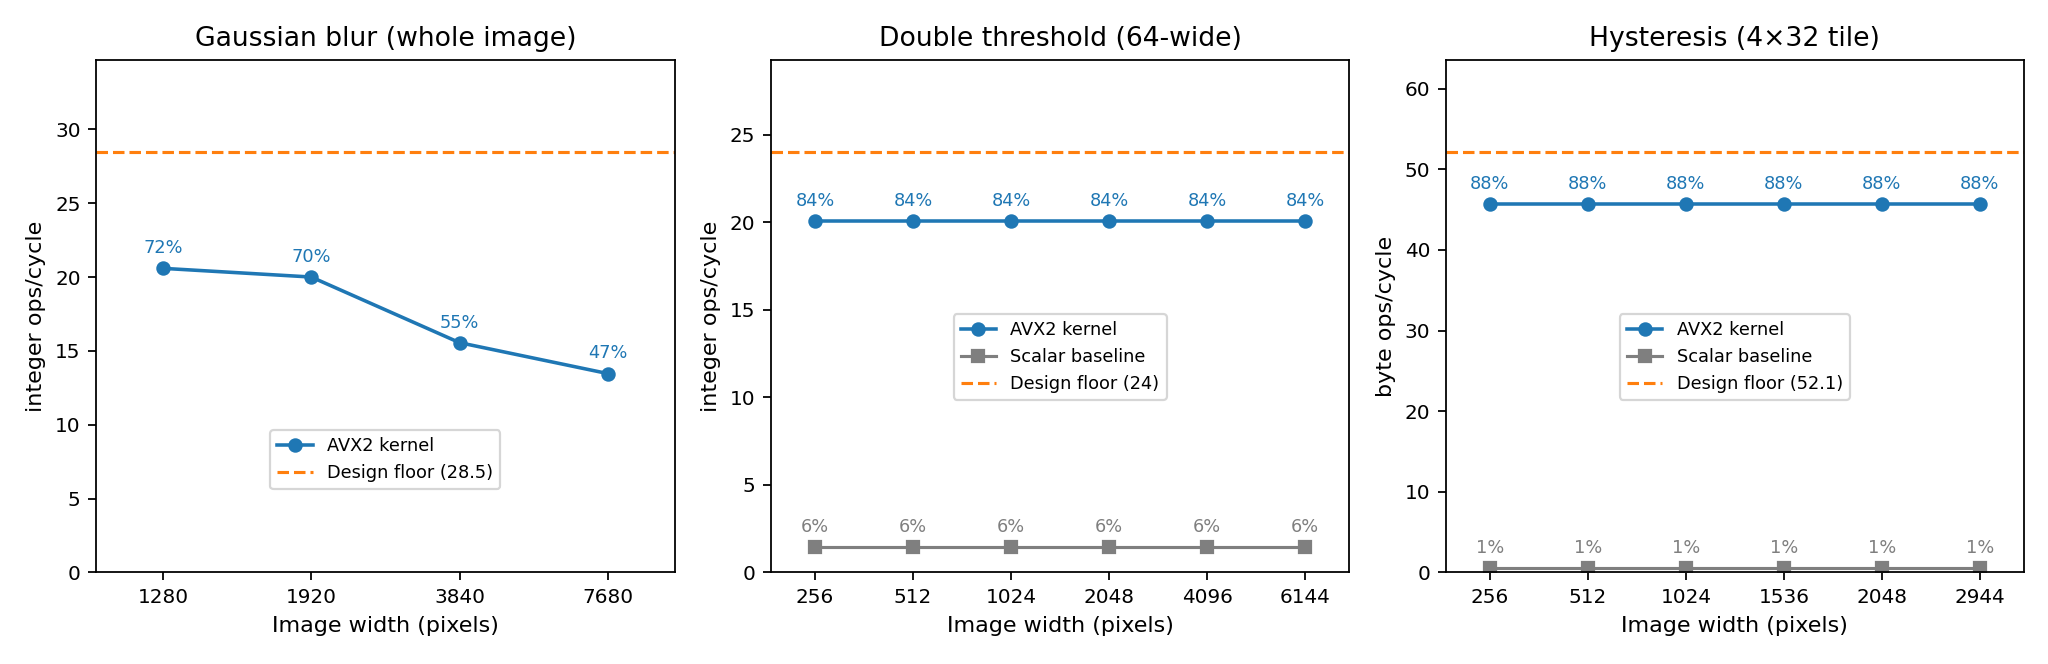
\includegraphics[width=\linewidth]{fig_performance_rest.png}\\
{\footnotesize Figure 2: The same three kernels against the design floors in the text (28.5 integer ops/cycle, 24 integer ops/cycle, and 52.1 byte ops/cycle). Labels are percent of that floor.
Gaussian is the whole-image table: 20.0 integer ops/cycle, 70\%, at 1080p. Double threshold is the flat L1 band, 82--86\%, drawn at its midpoint. Hysteresis is the flat L1 band, 86--90\%, drawn the same way.}
\end{center}
\textbf{(d)} At 1080p Gaussian is 20.0 integer ops/cycle, 70\% of its 28.5 floor. Double threshold stays at 20 integer ops/cycle, 84\% of 24, and the hysteresis vector pass at 46 byte ops/cycle, 88\% of 52.1.

\end{document}
